%%%% CAPÍTULO 1 - INTRODUÇÃO
%%
%% Deve apresentar uma visão global da pesquisa, incluindo: breve histórico, importância e justificativa da escolha do tema,
%% delimitações do assunto, formulação de hipóteses e objetivos da pesquisa e estrutura do trabalho.

%% Título e rótulo de capítulo (rótulos não devem conter caracteres especiais, acentuados ou cedilha)
\chapter{Introdução}\label{cap:introducao}

\section{TEMA}\label{sec:tema}
Segundo o Vocabulário Internacional de Metrologia, a metrologia é a ciência da medição e suas aplicações. Ela engloba todos os aspectos teóricos e práticos da medição, qualquer que seja a incerteza de medição e o campo de aplicação \cite{linck}.

Para efeito de medição, são utilizados diversos instrumentos, dependendo da área de atuação e também dos parâmetros desejados. Existem medidores de temperatura, de PH, balanças digitais, espectrofotômetros, cromatógrafos, entre vários outros instrumentos de medição. O escopo de atuação deste trabalho está limitado a equipamentos de medição de múltiplas grandezas elétricas denominados multímetros. Existem multímetros tanto analógicos quanto digitais.

O multímetro digital é a ferramenta padrão utilizada por profissionais nas áreas de elétrica ou eletrônica, principalmente, para medir tensão, corrente e resistência, podendo este ter funções adicionais dependendo do fabricante.

Tão cedo quanto 1950, foram feitas as primeiras iterações do multímetro digital, sendo a primeira versão portátil e confiável fabricada pela Fluke, em 1977, com o modelo 8020A, que revolucionou a indústria \cite{DMMHistory}. Desenvolvidos com a expectativa de leituras mais precisas, maior confiabilidade, robustez e menores preços, este equipamento começou a ser estudado para substituir o voltímetro, amperímetro, ohmímetro, e também os multímetros analógicos. 

Com a evolução da tecnologia, existe a possibilidade da utilização de computadores junto aos instrumentos de medição, tornando-os ainda mais práticos, fornecendo também a possibilidade de armazenamento e tratamento dos dados obtidos.

No curso de Engenharia Elétrica da \gls{utfpr} (Universidade Tecnológica Federal do Paraná), a primeira interação dos alunos com instrumentos de medição, mais especificamente o multímetro digital, é feita nas disciplinas de Eletricidade e Magnetismo e Circuitos Elétricos A. Os laboratórios de tais disciplinas e algumas outras serão o ponto focal da utilização dos dispositivos neste trabalho desenvolvidos.

\subsection{Delimitações do tema}\label{subsec:del-tema}
Para o desenvolvimento de um multímetro capaz de ler diversos canais de maneira isolada seria necessária a utilização de tecnologias de maior custo. Sendo necessária a utilização de amplificadores operacionais isolados ou transformadores de corrente com múltiplos taps para manter-se a precisão do dispositivo.

Dessa maneira, para que o dispositivo mantenha-se de baixo custo, este será feito de maneira modular, possuindo apenas um canal de tensão e um canal de corrente isolados entre si. Sua modularização se dará da possibilidade de utilizar mais de um multímetro em paralelo --- medindo um canal extra de tensão e corrente para cada adição --- com seus sinais sincronizados através de um circuito acessório que os interconecta e, também, por software.

Existem vários modos de se projetar uma fonte adequada ao sistema proposto, mas para o escopo deste trabalho, foi optado por se utilizar uma fonte comercial que será escolhida para atender as necessidades do protótipo em questão.

\section{PROBLEMA E PREMISSAS}\label{sec:probpremiss}
A Universidade Tecnológica Federal do Paraná - campus Curitiba, possui dois laboratórios de ensino para as disciplinas de Eletricidade e Magnetismo, Circuitos Elétricos A e B, ofertadas por diversos cursos da universidade. Os laboratórios são salas com bancadas de testes para circuitos elétricos que possuem fontes de tensão e corrente, bem como módulos de medidores para diversos fins.

Esses medidores, porém, são completamente analógicos, possuem fundo de escala que não condizem necessariamente com os testes que precisam ser realizados durante as aulas práticas e, muitas vezes, não estão em condições adequadas de funcionamento. Isso se dá em grande parte por sua complexidade de reparos: tanto por necessitarem peças antigas para reposição, quanto por possuírem diversas peças mecânicas em seu interior que dificultam o processo de reparo, demandando muito tempo e realização de testes, como calibração posterior; além de não possuírem sistemas de proteção adequados para o uso em sala de aula – local em que o aparelho sofre desgaste por erros comuns da prática de discentes.

Adicionalmente, há também a questão de custos de aquisição de módulos novos que se adequem às bancadas utilizadas nos laboratórios e ao tipo de uso. Há uma grande limitação sobre o número de dispositivos disponíveis, dado os valores de medidores encontrados no mercado e disponibilidade de recursos da universidade.

\section{OBJETIVOS}\label{sec:objetivos}

\subsection{Objetivo Geral}\label{sec:objgeral}
Desenvolvimento de um multímetro modular com comunicação sem fio de baixo custo para laboratórios da \gls{utfpr}.


\subsection{Objetivos Específicos}\label{sec:objespec}
Projetar um multímetro de baixo custo modular capaz de medir tensão e corrente \gls{CC}/\gls{CA} simultaneamente, com proteções contra curto-circuito e sobretensão. Tal equipamento também se comunicará com um smartphone por protocolo \textit{wireless} para apresentar as formas de onda e dados obtidos das medições para ser utilizado nos laboratórios das disciplinas de Eletricidade e Magnetismo, Circuitos Elétricos A e B da \gls{utfpr} – câmpus Curitiba.

Para o desenvolvimento do multímetro, serão necessários os seguintes processos:

\begin{itemize}
    \item Levantar, juntamente dos professores que utilizam os laboratórios e que utilizarão o equipamento, quais as necessidades físicas, parâmetros de medida, e níveis de tensão e corrente necessários para atender os requerimentos das práticas experimentais;
    \item Verificar quais são os métodos comumente utilizados por equipamentos profissionais para proteção e amostragem de dados;
    \item Definir as funções específicas do equipamento;
    \item Listar os materiais necessários para a construção do equipamento;
    \item Escolher os softwares e protocolos a serem utilizados para o desenvolvimento do projeto;
    \item Desenvolver de um protótipo funcional do multímetro modular;
    \item Desenvolver um sistema de fixação e alimentação para sua instalação nas bancadas de laboratório e;
    \item Realizar o teste do protótipo.
\end{itemize}

\section{JUSTIFICATIVA}\label{sec:justificativa}
Uma ferramenta de medição de baixo custo, com capacidade de atender às principais demandas de obtenção de dados, proteção e simplicidade de reparos, bem como a possibilidade de replicabilidade de maneira simples, poderia facilitar o dia a dia dos usuários dos laboratórios de aulas práticas e tornar o ensino mais dinâmico e adequado à prática almejada, estendendo a experiência de ensino das disciplinas através do tratamento de dados de maneira mais específica e observação simultânea das formas de onda.

\section{METODOLOGIA DE PESQUISA}\label{sec:metodologiapesq}
Este \gls{TCC} se trata de uma pesquisa exploratória aplicada que visa o desenvolvimento de um protótipo de um multímetro digital com suas especificidades e testes para assegurar sua viabilidade. 
Para a elaboração deste trabalho será necessário compreender melhor o problema que os professores das disciplinas de circuitos da \gls{utfpr} enfrentam com os equipamentos de medição disponíveis para as aulas. Aplicar questionários sobre quais medições seriam mais importantes e quais proteções deveriam ser consideradas para os mesmos.
Será necessário desenvolver um sistema elétrico, mecânico (carcaça) e um software para a interação do usuário com o medidor. Isso demandará um estudo dos componentes a serem utilizados, bem como definir quais programas e ferramentas de desenvolvimento serão necessários para cada uma das áreas.
Também sobre o equipamento, pesquisar-se-á métodos de amostragem utilizados em produtos comerciais e aprofundar os conhecimentos nos microcontroladores, componentes e plataformas de desenvolvimento escolhidos.

\section{ESTRUTURA DO TRABALHO}\label{sec:estruturatrab}

Para atingir os objetivos geral e específicos, este trabalho será estruturado da seguinte forma:

\begin{itemize}
    \item Capítulo 01: Introdução do tema, motivação e dos objetivos.
    \item Capítulo 02:
    \item Capítulo 03:
    \item Capítulo 04:
\end{itemize}

\section{CRONOGRAMA}\label{sec:cronogramsboi}

\begin{figure}[htb!]
    \caption{Cronograma do Trabalho de Conclusão de Curso}
    \label{fig:cronograma}
    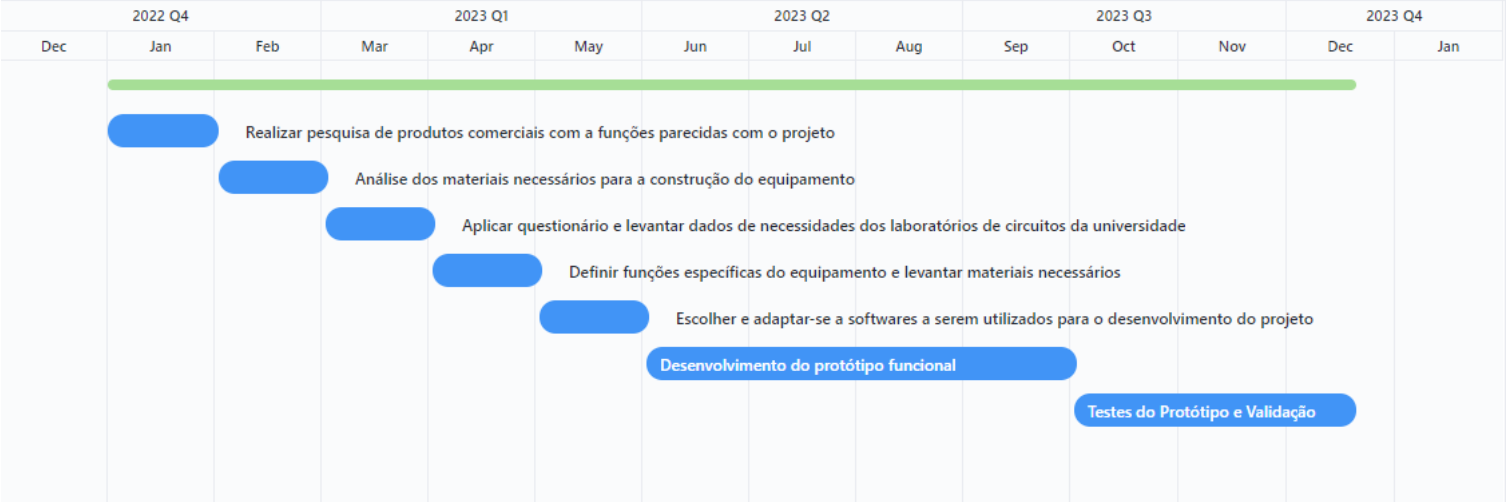
\includegraphics[width=0.8\textwidth]{figuras/gantt-cronograma.png}
    \fonte{}
\end{figure}